\documentclass[a4paper,12pt]{article}
\usepackage[utf8]{inputenc}
\usepackage[T1]{fontenc}
\usepackage[hungarian]{babel}
\usepackage{graphicx}
\usepackage{geometry}
\geometry{a4paper,
		     tmargin = 35mm, 
		     lmargin = 25mm,
		     rmargin = 30mm,
		     bmargin = 30mm}
\usepackage{mathtools}
\usepackage{amsmath}
\usepackage{color}
\usepackage{setspace}
\usepackage{amsmath,amssymb}
\usepackage{float}
\usepackage{hyperref}

\usepackage{indentfirst}
\usepackage{subfig}

\usepackage{siunitx}

\renewcommand\thesection{\Roman{section}}

\begin{document}

\linespread{1.25}

\begin{titlepage}

	\centering
	
\includegraphics[width=0.66\textwidth]{elte.jpg}\par\vspace{1cm}
	{\scshape\LARGE ELTE TTK \par}
	\vspace{3cm}
	{\scshape\Large Meissner-effektus vizsgálata \par}
	\vspace{1cm}
	{\large\itshape Olar Alex\par}
	\vspace{3cm}
	{\large 2018 \par}
	
\end{titlepage}

\tableofcontents

\newpage

\section{Elméleti összefoglaló, mérési eszközök}

\vspace{5mm}

\par A szupravezető anyagra jellemző hőmérséklet alatt kizárja magából a mágneses teret. Az adott anyag ekkor tökéletes diamágnessé válik, azaz a mágneses szuszceptibilitása, $\chi = -1$ lesz. A kísérlet során ennek változásást vizsgáljuk. A ténylegesen mért $\chi$ érték nem lesz természetesen $-1$, mivel nem válik az anyag egésze szupravezetővé.

\vspace{5mm}

\par A mérés során sorosan kötött tekercsek közitti platina hőmérővel mérjük a hőmérsékletet. A tekercsek közötti kis feszültségkülönbséget pedig a minta nélküli tekercsre kötött műveleti erősítőből a lock-in műszerre kötve mérjük. Így a mintát behelyezve az egyik tekercsbe az feszültségkülönbséget okoz a két tekercs között:

\begin{equation}
	\frac{\Delta U}{U_{0}} = \chi \frac{V_{m}}{V}
\end{equation} 

\par Esetünkben a jegyzethez képest egy negatív előjel különbég van, mivel ellentétesen kalibráltuk a szuszceptibilitás-feszültség kitérést. A lock-in kimenetén lévő feszültség maximumát és minimumát megkeresve, minta nélkül, bekalibráltuk azt $90^{\circ}$-ra, azaz (d) ponton mért $0 ~V$-ra, természetesen ezén még volt egy offset feszültség, amit részben külső, részben belső fázistolás okozott. 

\begin{figure}[!htb]
\centering
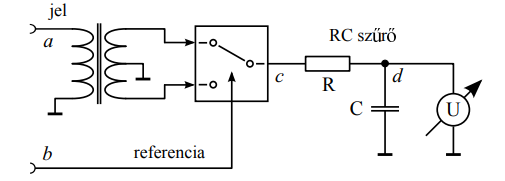
\includegraphics[width=0.35\textwidth]{./lockin.png}
\caption{A lock-in műszer vázlatos rajza, és a $(d)$ ponton mért feszültség}
\end{figure}

\par A mérési adatokat egy számítógép mentette nekünk, minden pontban egy hőmérséklet, feszültség, idő és melegedés/hűlés számkódot kaptunk meg. A lock-in műszer feszültségállásából mindi tudnunk kellett az aktuális méréshatárt. Ez a Meissner-effektus során $300 ~\mu V$-ra volt állítva, míg $U_{0}$ mérése során $10 ~mV$-ra. Ebből $U_{0}$ mért értékére:

\begin{equation}
U_{0} = (5.74 \pm 0.01) ~mV 
\end{equation}

\par Az adatok közül ismert volt $V$ és $V_{m}$, amelyek $(1)$-ben szerepelnek. Ezek rendre $300 ~mm^{3}$ és $22 ~mm^{3} \pm 1\%$ térfogatúak. Így a kapott feszültség-hőmérséklet diagrammokat szuszceptibilitás-hőmérséklet diagrammokká lehetett konvertálni.

\subsection{Hibabecslés}

\par A szuszceptibilitás hibájához figyelmbe kell venni a $U_{0}$ mérési hibáját és a minta térfogatának hibáját, amik rendre 1\% és 0.1\%. A feszültség mérés bizonytalánságát figyelembe véve azonban a szuszceptibilitás hibáját 2\%-al becsülöm. Ezen kívül még a hőmérséklet mérésnek $0.5~K$ körüli hibát becsülök, mivel a platina hőmérő nem közvetlenül a mintát méri, hanem a két tekercs között helyezkedik el.

\section{ Kiértékelés}

\vspace{2mm}

\par Először is ábrázoltak a kérdéses tartományban a melegedéshez és hűléshez tartozó mérési pontokat.

\vspace{2mm}

\begin{figure}[!htb]
\centering
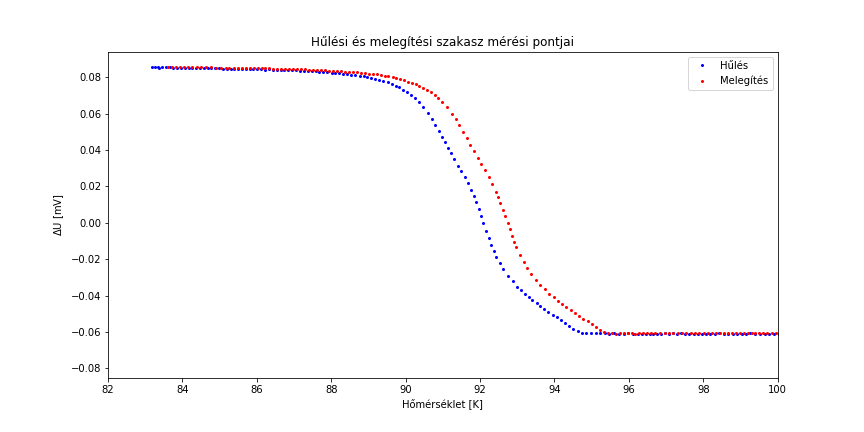
\includegraphics[width=.95\textwidth]{coolingAndHeating.png}
\end{figure}

\vspace{2mm}

\par A leírásban szerepel, hogy a legegyszerúbb módszer egyszerűen adott $T$ hőmérséklet mellett összeátlagolni a mérési eredményeket és ezáltal megszerkeszteni az átlagolt átmeneti görbét.

\vspace{2mm}

\begin{figure}[!htb]
\centering
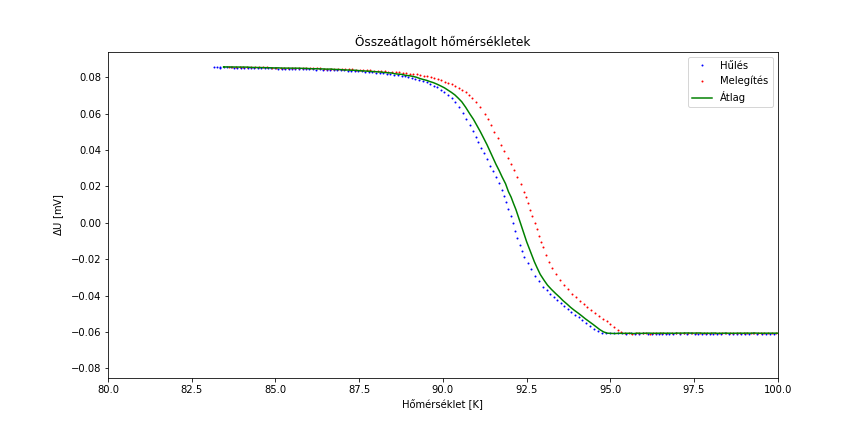
\includegraphics[width=.95\textwidth]{coolingAndHeatingWithMean.png}
\end{figure}

\vspace{2mm}

\par Azonban itt figyelmbe kell venni a melegedés sebességét, amit szintén az adatsorban megkaptunk. Véve tehát először a hőmérséklet-idő grafikonokat hűlésre és melegedésre a következőt kaptam:

\vspace{2mm}

\begin{figure}[!htb]
\centering
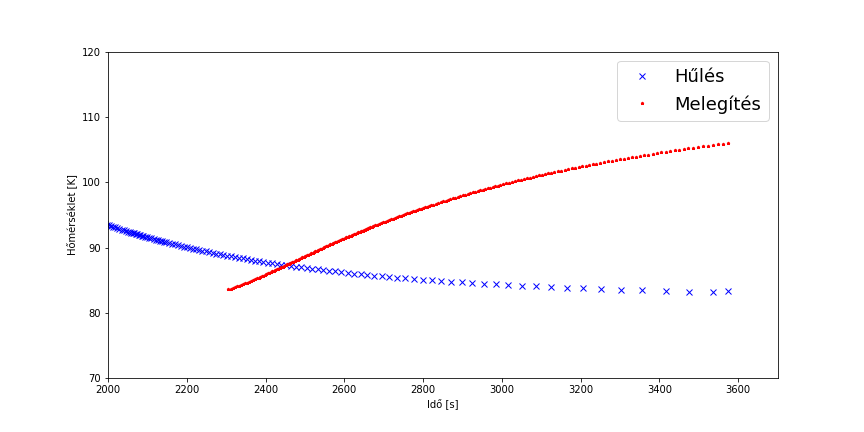
\includegraphics[width=.95\textwidth]{tempCoolingHeating.png}
\caption{ A melegedés időben vissza van tolva hiszen a hűlés hőmérséklete után kezdődött el és ment végig ugyan azon az átmeneti hőmérséklet tartományon  }
\end{figure}

\vspace{2mm}

\par Ahol látható, hogy a görbék meredeksége jócskán eltér, így azok meredekségével súlyozva számoltam ténylegesen összeátlagolt görbét. Ehhez persze deriválni kellett az előbbi görbéket. Természetesen diszkrét esetben differenciát vettem:

\vspace{2mm}

\begin{figure}[!htb]
\centering
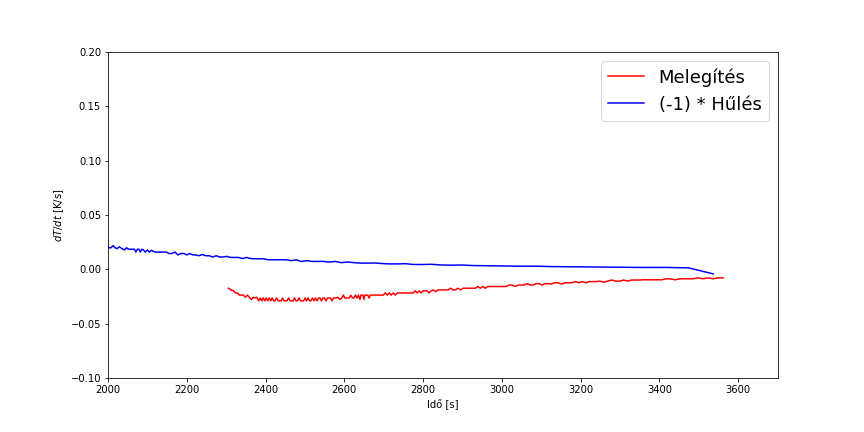
\includegraphics[width=.95\textwidth]{derivTempCoolingHeating.png}
\end{figure}

\vspace{2mm}

\par Ahol a hűlés deriváltjának $(-1)$-szeresét vettem, mert abszolútértékben kell súlyoznom. Ezzel a következő eredményre 
jutottam:

\vspace{2mm}

\begin{figure}[!htb]
\centering
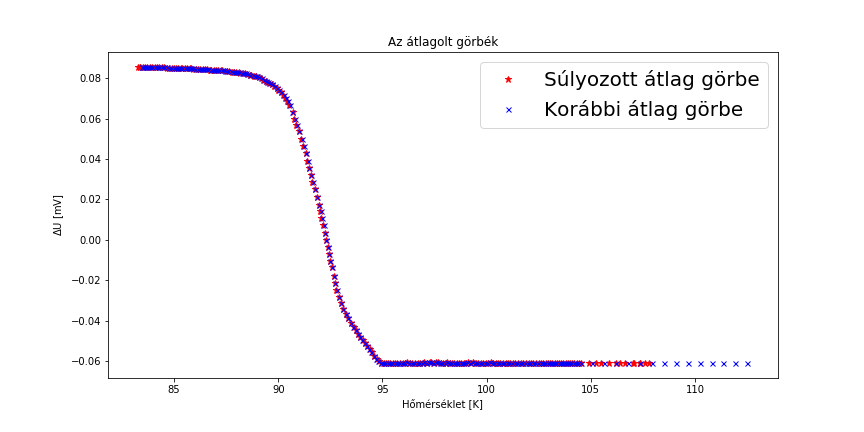
\includegraphics[width=.95\textwidth]{weightedMeanPlot.png}
\caption{A korábbi, egyszerűen összeátlagolt görbe, és a meredekségekkel súlyozottan összeátlagolt görbe}
\end{figure}

\vspace{2mm}

\par Látható, hogy az eltérés valójában közel elhanyagolható, hiába a derváltak közötti eltérés. Az a helyzet, hogy ilyen pontosan mint amennyit ez javít az átlagon nem fogom a szuszceptibilitást megmondani. Ennek ellenére a súlyozott görbét konvertálom az $(1)$-es egyenlettel a szuszceptibilitás-hőmérsékletté:

\vspace{2mm}

\begin{figure}[!htb]
\centering
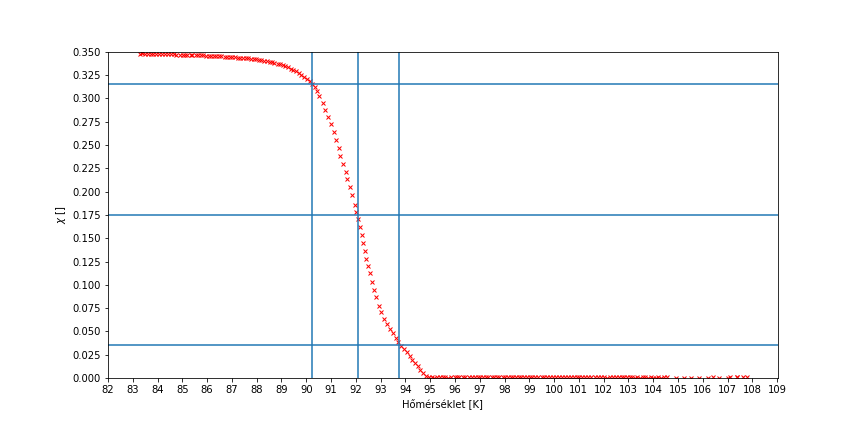
\includegraphics[width=1\textwidth]{szuszcepti.png}
\caption{Az átlagolt görbe transzformáltja, a 10\%-os és 90\%-os szuszceptibilitásértkeknél jelzett kék vonalak metszétpontjaival, míg a középső az átlagakulás $T_{c}$ hőmrésékletét hivatott jelezni}
\end{figure}

\vspace{2mm}

\par A kék vonalak $T_{1} = (90.25 \pm 0.5) ~K$ és $T_{2} = (92.75 \pm 0.5) ~K$-nél metszik a görbét. A szuszceptibilitás maximális értéke jól láthatóan $ \chi = -( 0.35 \pm 0.01) $, míg természetesen az offset miatt kellett bevinnem a rendszerbe egy $0.145$-ös eltolást, hogy $95~K$ felett, $0$-ba kalibráljam a mérést. Az átalakulás hőmérséklet a szuszceptibilitás 50\%-os értékéhez kalibrálva $T_{c} = (92.1 \pm 0.5) ~K$.

\end{document}